% Chapter 5

\chapter{Benchmark results and discussion} % Main chapter title
\label{Results} % For referencing the chapter elsewhere, use \ref{Chapter1} 

\lhead{Chapter \ref{Results}. \emph{Benchmark results and discussion}} % This is for the header on each page - perhaps a shortened title

Chapter \ref{CUDAHMMER3} described several approaches to optimize the cudaHmmsearch implementation. This chapter presents the performance measurements when experimenting these approaches on a GPU and on a multicore CPU.
%----------------------------------------------------------------------------------------

\section{Benchmarking environment}
The benchmarking environment were set up in Kronos machine \label{Kronos}as follows:
 
\begin{itemize}
 \item CPU host\\
 Intel� Core� i7-3960X with 6 cores, 3.3GHz clock speed, 64GB RAM
 \item GPU device\\
 NVIDIA� Quadro� K4000 graphics card with 3 GB global memory, 768 Parallel-Processing Cores, 811 MHz GPU Clock rate, CUDA Compute Capability 3.0.
 \item Software system\\
 The operating system used was Ubuntu 64 bit Linux v12.10; the CUDA toolkit used was version 5.5.
 \item Target sequences database\\
 One was Swiss-Prot database in fasta format released in September 2013 \citep{UniProt} containing 540,958 sequences with length varying from 2 $\sim$ 35,213 amino acids, comprising 192,206,270 amino acids in total, more than 258MB in file size. Another was much larger NCBI NR database in fasta format released in April 2014 \citep{NCBI} containing 38,442,706 sequences with length varying from 6 $\sim$ 41,943 amino acids, comprising 13,679,143,700 amino acids in total, more than 24GB in file size.
 \item Query profile HMMs\\
 We tested 5 profile HMMs of length 149, 255, 414, 708 and 1111 states, detailed in Table\ref{tab.phmms}. Globin4 with length of 149 states was distributed with the HMMER source \citep{Hsource}. Other 4 HMMs were taken directly from the Pfam database \citep{Pfam} that vary in length from 255 to 1111 states.\\
 \begin{table}[H]
 \centering
 \begin{tabular}{|c|c|c|c|c|c|}\hline
 \textbf{Name} & Globin4 & 120\_Rick\_ant & 2HCT & ACC\_central & AAA\_27 \\\hline
 \textbf{Accession number} & - & PF12574.3 & PF03390.10 & PF08326.7 & PF13514.1 \\\hline
 Length & 149 & 255 & 414 & 708 & 1111 \\\hline
 \end{tabular}
 \caption{\fontfamily{pag}\selectfont Profile HMMs used in benchmarking. \label{tab.phmms} Globin4 has no Accession number.}
 \end{table}
 \item Measuring method\\
 The execution time of the application was timed using the C clock() instruction. The performance was measured in unit GCUPS(Giga Cell Units Per Second) which is calculated as follows:
 \begin{equation*}
   GCUPS = \frac{L_q * L_t}{T * 1.0e09}
 \end{equation*}
 where $L_q$ is the length of query profile HMM, i.e. the number of the HMM states, $L_t$ is the total residues of target sequences in the database, $T$ is the execution time in second.\\
 All programs were compiled using GNU g++ with the -O3 option and executed independently in a 100\% idle system.
\end{itemize}

%----------------------------------------------------------------------------------------

\section{Performance Results}

\subsection{Comparison with less optimized approaches}
To show the performance impact of several selected optimization approaches, the performance of the implementation was compared with that of previous approach.

Table\ref{tab.opt} shows the approaches taken in optimizing performance. All tests are taken against the Swiss-Prot database. The query HMM used was globin4. The fourth column `Improvement' is measured in percentage compared with the previous approach.

\begin{table}[H]
\centering
\begin{tabular}{|c|c|c|c|}\hline
\shortstack{\textbf{Description of} \\ \textbf{approach}} & \shortstack{\textbf{Execution} \\ \textbf{time (s)}} & \shortstack{\textbf{Performance}\\ (GCUPS)} & \shortstack{\textbf{Improvement}\\ \textbf{(\%)}}\\\hline
Initial implementation & 227.178 & 0.126 & - \\\hline
SIMD Video Instruction& 125.482 & 0.228 & 81 \\\hline
\shortstack{Minimizing global\\memory access} & 16.449 & 1.741 & 664 \\\hline
\shortstack{Async memcpy \&\\Multi streams} & 9.463 & 3.026 & 74 \\\hline
\shortstack{Coalescing of\\global memory} & 6.565 & 4.362 & 44 \\\hline
Texture memory & 5.370 & 5.333 & 22 \\\hline
Sorting Database & 2.346 & 12.207 & 129 \\\hline
Distributing workload & 1.650 & 17.357 & 42 \\\hline
\end{tabular}
\caption{\fontfamily{pag}\selectfont \textbf{Performance of optimization approaches.} The fourth column \textbf{Improvement} is measured in percentage compared with the previous approach. The row `Coalescing of global memory' is benchmarked only for the $dp$ matrix. The row `Texture memory' is benchmarked only for the query profile texOMrbv 2D texture. \label{tab.opt}}
\end{table}

The graphic view corresponding to Table is shown in Figure\ref{fig:imp}. 

\begin{figure}[!htb]
	\centering
	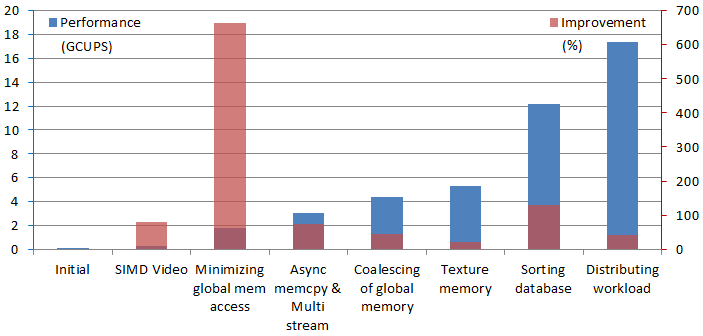
\includegraphics[totalheight=0.28\textheight]{Figures/improve.png}
	\caption{\fontfamily{pag}\selectfont \textbf{Performance of optimization approaches.} The data of this chart come from Table\ref{tab.opt}. The blue bar is Performance (in GCUPS) of each approach, corresponding to the left Y axis. The red bar is Improvement in \% corresponding to the right Y axis.}
	\label{fig:imp}
\end{figure}

From the chart, it can be seen that several factors are related to global memory accesses, including the highest 663\% minimizing global memory access, coalescing of global memory and texture memory. So the global memory optimizations are the most important area for performance. To make all threads in a warp execute similar tasks, the auxiliary sorting database also plays important role in optimizations.

\subsection{Practical benchmark}
\label{Pbench}
The final cudaHmmsearch implementation, with the optimization discussed in Chapter\ref{CUDAHMMER3}, was benchmarked to determine its real-world performance. This was done by searching the much large NCBI NR database for the 5 profile HMMs with various lengths, as detailed in Table\ref{tab.phmms}. As comparison, the same searches were executed by hmmsearch of HMMER3 on 1 CPU core. The result of this benchmark is shown in the following table.

\begin{table}[H]
\centering
\begin{tabular}{|c|c|c|c|c|c|}\hline
\shortstack{\textbf{Profile HMM} \\ \textbf{(length)}} & \shortstack{\textbf{globins4} \\ (149)} & \shortstack{\textbf{120\_Rick\_ant}\\ (255)} & \shortstack{\textbf{2HCT}\\ (414)} & \shortstack{\textbf{ACC\_central} \\ (708)} & \shortstack{\textbf{AAA\_27} \\ (1111)} \\\hline
\shortstack{Performance of \\ hmmsearch \\ (GCUPS)} & 9.37 & 11.72 & 11.68 & 11.96 & 6.90 \\\hline
\shortstack{Performance of \\ cudaHmmsearch \\ (GCUPS)} & 23.00 & 32.17 & 30.01 & 32.83 & 14.68 \\\hline
\shortstack{Speedup \\ (times)} & 2.45 & 2.74 & 2.57 & 2.75 & 2.13 \\\hline
\end{tabular}
\caption{\fontfamily{pag}\selectfont \textbf{Result of Practical benchmark.} \label{tab.pb} Speedup is measured in times of cudaHmmsearch performance over that of hmmsearch.}
\end{table}

The results of the benchmarks are shown in graphical form in Figure\ref{fig:len}. The GPU cudaHmmsearch performance hovers just above 25 GCUPS, while the CPU hmmsearch only around 10 GCUPS. The whole performance of cudaHmmsearch is stable with various lengths of query HMMs. On average, cudaHmmsearch has a speedup of 2.5x than hmmsearch. 

\begin{figure}[!htb]
	\centering
	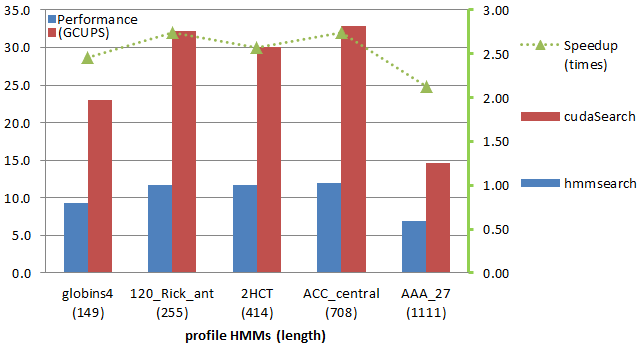
\includegraphics[totalheight=0.36\textheight]{Figures/lengths.png}
	\caption{\fontfamily{pag}\selectfont \textbf{Practical benchmarks.} The data of this chart come from Table\ref{tab.pb}. The blue and red bar is Performance (in GCUPS) of hmmsearch and cudaHmmsearch respectively, corresponding to the left Y axis. The green dot line is Speedup (in times) of cudaHmmsearch performance over that of hmmsearch, corresponding to the right Y axis.}
	\label{fig:len}
\end{figure}

Figure\ref{fig:len} shows that the performance of both GPU and CPU searching for AAA\_27 dropped greatly. The reason can be seen from the table\ref{tab.sta} listing the internal pipeline statistics summary for searching globin4 and AAA\_27. For every filter, the count of passed sequences for searching AAA\_27 with 1111 states is much more than that of globin4 with 149 states. This means that for searching AAA\_27, much more target sequences than searching globin4 are needed calculating in each filter after MSV filter. And at the same time, each filter is more time-consuming than MSV filter. All of these result in the AAA\_27 performance dropping greatly.

\begin{table}[H]
\centering
\begin{tabular}{|c|c|c|}\hline
\shortstack{\textbf{Query profile HMM(length)}} & \shortstack{\textbf{globin4 (149 states)}} & \shortstack{\textbf{AAA\_27 (1111 states)}}\\\hline
Target sequences & 38442706 & 38442706 \\\hline
Passed MSV filter & 1195043 & 4305846 \\\hline
Passed bias filter & 973354 & 1671084 \\\hline
Passed Viterbi filter & 70564 & 322206 \\\hline
Passed Forward filter & 7145 & 17719 \\\hline
\end{tabular}
\caption{\fontfamily{pag}\selectfont Internal pipeline statistics summary\label{tab.sta}}
\end{table}

\subsection{Comparison with multicore CPU}
Since multicore processors were developed in the early 2000s by Intel, AMD and others, nowadays CPU has become multicore with two cores, four cores, six cores and more. The Kronos \ref{Kronos} experiment system has CPU with six cores. This section presents the benchmarks of cudaHmmsearch running with multiple CPU cores.

The experiment was done by executing cudaHmmsearch and hmmsearch with 1, 2...6 CPU cores, searching the NCBI NR database for the HMM with 255-state length.

The benchmark has not been used in the articles cited in this thesis. The purpose of this benchmark is to show how the performance increase or decrease with more CPU cores involved in computing. The result of this benchmark is shown in the following table.

\begin{table}[H]
\centering
\begin{tabular}{|c|c|c|c|c|c|c|}\hline
\shortstack{\textbf{Performance} \\ \textbf{(GCUPS)}} & \shortstack{1 CPU \\ core} & \shortstack{2 CPU \\ cores} & \shortstack{3 CPU \\ cores} & \shortstack{4 CPU \\ cores} & \shortstack{5 CPU \\ cores} & \shortstack{6 CPU \\ cores} \\\hline
cudaHmmsearch & 32.17 & 50.22 & 57.70 & 59.14 & 59.39 & 59.29 \\\hline
hmmsearch & 11.72 & 23.28 & 29.22 & 44.15 & 46.19 & 44.69 \\\hline
\end{tabular}
\caption{\fontfamily{pag}\selectfont {Result of Comparison with multicore CPU.} \label{tab.mcpu}}
\end{table}

The graphic view of the benchmark is shown in Figure\ref{fig:cpuCores}. The number above each bar is the Performance in GCUPS. As can be seen, from 1 CPU core to 4 CPU cores, both cudaHmmsearch performance and hmmsearch performance go up almost linearly. From then on, due to complex schedule among CPU cores, the extra CPU core will not contribute much to both cudaHmmsearch and hmmsearch execution. Even worse, it will have negative effect as shown clearly in the `6 CPU' case.

\begin{figure}[!htb]
	\centering
	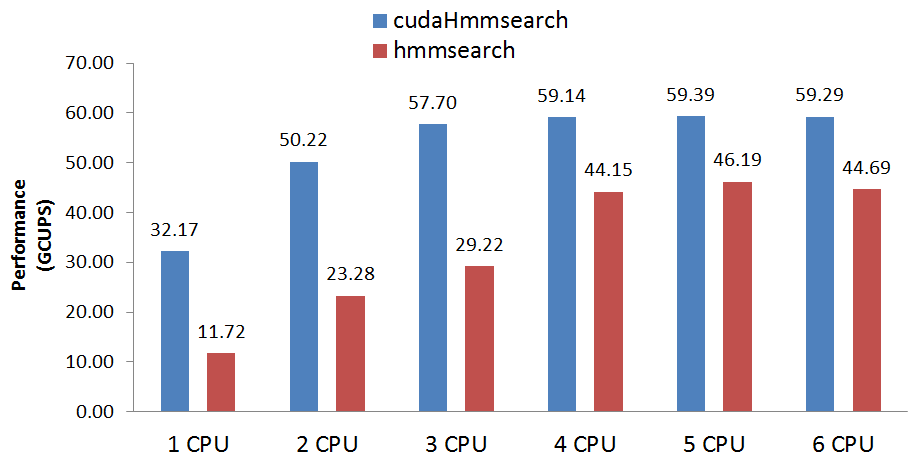
\includegraphics[totalheight=0.25\textheight]{Figures/cpuCores.png}
	\caption{\fontfamily{pag}\selectfont \textbf{Comparison with multicore CPU.} The data of this chart come from Table\ref{tab.mcpu}. The number above each bar is the Performance in GCUPS.}
	\label{fig:cpuCores}
\end{figure}

\subsection{Comparison with other implementations}
The performance of cudaHmmsearch was also compared to the previous HMMER solutions: HMMER2.3.2 \citep{HMMER2}, GPU-HMMER2.3.2 \citep{GPUHMM} and HMMER3 \citep{Hsource}.

All tests are taken searching against the Swiss-Prot database for the globin4 profile HMM. The result of this benchmark is shown in the following table.

\begin{table}[H]
\centering
\begin{tabular}{|c|c|c|c|c|}\hline
\shortstack{Application \\ (Device)} & \shortstack{HMMER2.3.2 \\ (CPU)} & \shortstack{GPU-HMMER2.3.2 \\ (GPU)} & \shortstack{HMMER3 \\ (CPU)} & \shortstack{cudaHmmsearch \\ (GPU)} \\\hline
\shortstack{Performance\\ (GCUPS)} & 0.14 & 0.95 & 8.47 & 17.36 \\\hline
\end{tabular}
\caption{\fontfamily{pag}\selectfont {Result of Comparison with other implementations.} \label{tab.hmms}}
\end{table}

As seen from the Figure\ref{fig:hmms}, since the release of HMMER2.3.2 in Oct 2003, accelerating hmmsearch researches on both CPU and GPU have achieved excellent improvement.

\begin{figure}[!htb]
	\centering
	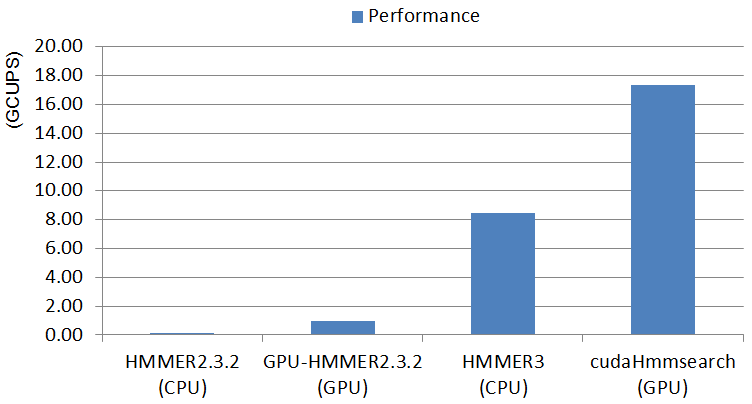
\includegraphics[totalheight=0.28\textheight]{Figures/manyhmms.png}
	\caption{\fontfamily{pag}\selectfont Comparison with other implementations.}
	\label{fig:hmms}
\end{figure}

%----------------------------------------------------------------------------------------

% Chapter 6

\chapter{Conclusions} % Main chapter title

\label{Conclusions} % For referencing the chapter elsewhere, use \ref{Chapter1} 

\lhead{Chapter \ref{Conclusions}. \emph{Conclusions}} % This is for the header on each page - perhaps a shortened title

A fully-featured and accelerated HMMER3 protein search tool \emph{cudaHmmsearch} was implemented on CUDA-enabled GPU. It can search the protein sequence database for profile HMMs.

%----------------------------------------------------------------------------------------

\section{Summary of Contributions}
Our research work started with dynamic programming, the common characteristic of Swith-Waterman algorithm, Viterbi algorithm and MSV algorithm, which are famous protein sequence alignment algorithms in Bioinformatics.
We specially summarized the technologies of accelerating Swith-Waterman algorithm on CUDA-enabled GPU, on which has been widely researched. We also briefly presented GPU acceleration work related to Viterbi algorithm.

After analyzing the core application \emph{hmmsearch} in HMMER3, we found the key hotspot MSV filter for accelerating hmmsearch. We presented the details of our \emph{cudaHmmsearch} implementation and optimization approaches. At the same time, we also discussed and analyzed the advantages and limitations of GPU hardware for CUDA parallel programming. Then we summarized 6 steps for better performance of CUDA programming.

We performed comprehensive benchmarks. The results were analyzed and the efficiency of the \emph{cudaHmmsearch} implementations on the GPUs is proved. We achieved 2.5x speedup over the single-threaded HMMER3 CPU SSE2 implementation. The performance analysis showed that GPUs are able to deal with intensive computations, but are very sensitive to random accesses to the global memory.

The solutions in this thesis were designed and customized for current GPUs, but we believe that the principles studied here will also apply to future manycore GPU processors, as long as the GPU is CUDA-enabled. Here is the complete list of CUDA-enabled GPUs: \url{https://developer.nvidia.com/cuda-gpus}.

%----------------------------------------------------------------------------------------

\section{Limitations of Work}
There are some weak points in our work summarized as follows:

Although our \emph{cudaHmmsearch} can search against unsorted protein sequence database, it can gain 129\% improvement searching against sorted database according to benchmark Table\ref{tab.opt}. And although the extra sorting database program is provided, user may be unaware of this and run \emph{cudaHmmsearch} against an unsorted database. It is better for the program to evaluate the database automatically and prompt user to sort if necessary.

We use block reading method to process very large database. However, the number of sequences for each block reading is fixed. So the number of threads launched in GPU kernel is also fixed. For those sequences with shorter lengths, it is better to use dynamic block reading to get more sequences, so as to increase the occupancy of GPU threads and achieve better performance.

%----------------------------------------------------------------------------------------

\section{Recommendations for Future Research}
The limitations noted in the last section call attention to several areas that we deem worthy of further improvement and investigation. The suggested topics are placed under the following headings.

\subsection*{Forward filter for no threshold}
By default, the top-scoring of target sequences are expected to pass each filter. Alternatively, the -\emph{-max} option is available for those who want to make a search more sensitive to get maximum expected accuracy alignment. The option causes all filters except Forward/Backward algorithm to be bypassed. And according to practical benchmarking in Section\ref{Pbench}, the performance decreased greatly due to much more calculation in Forward algorithm. So our next research should be focused on accelerating Forward algorithm on CUDA-enabled GPU.

\subsection*{Multiple GPUs approach}
Since currently we don't have multiple GPUs within a single workstation, we didn't research on multiple GPUs approach. However, CUDA already provides specific facilities for multi-GPU programming, including threading models, peer-to-peer, dynamic parallelism and inter-GPU synchronization, etc. Almost all PCs support at least two PCI-E slots, allowing at least two GPU cards to insert almost any PC. Looking forward, we should also investigate multi-GPU solutions.

%----------------------------------------------------------------------------------------
